\chapter{Optimisers}
\label{chap:optimisation}
To actually train a model, we get some data and compute the loss based on the current model, as covered so far.
Then, we start an update step by finding the impact on the loss of changing the model parameters.
We do this by differentiating.
Once we have the dependence from the parameters on the loss, we need to decide how to actually update the parameter. 
To Our toolbox for this contains: information from previous steps, parameter scale and local curvature.

\section{Gradient Descent}

\label{sec:optimisation-gradient-descent-following-the-slope-downhill}
For model parameters $\theta\in\R^{N_{\text{parameters}}}$ and training loss $\mathcal L(\theta)$, gradient descent follows the local negative slope:
\begin{calloutmemorise}
\[
    \underbrace{\theta_{t+1}}_{\text{parameters after update}}
    =
    \underbrace{\theta_t}_{\text{current parameters}}
    -
    \underbrace{\eta}_{\text{learning rate}}
    \underbrace{\nabla_\theta\mathcal L(\theta_t)}_{\text{local uphill direction}}.
\]
\end{calloutmemorise}
The negative gradient is the steepest local descent direction for a fixed-length step measured using ordinary Euclidean distance.
The gradient says which way to move locally, but not how far its approximation remains useful.
A small $\eta$ makes slow progress; a large $\eta$ can cross a valley, oscillate, or diverge.

\begin{calloutexample}
    For $\mathcal L(\theta)=(\theta-3)^2$, every update moves relative to the same optimum at $\theta=3$.
    Changing only $\eta$ changes whether the iterates approach $3$ directly, alternate across it, or move away.
\end{calloutexample}

\figpdf[.98\textwidth]{gradient_descent_rates}{Gradient-descent step size on a quadratic loss: identical objective and start, different learning rates, different stability.}

\textbf{Curvature and Conditioning}
A gradient might be very symmetrically flat or sharply curved, where using the same learning rate in both directions causes slow progress in one and unstable steps in the other.
For a positive-definite quadratic loss with \textbf{Hessian} (second derivative, which shows curvature) $\nabla_\theta^2\mathcal L$, a fixed step is stable when
\[
    0<\underbrace{\eta}_{\text{step size}}
    <\frac{2}{\underbrace{\lambda_{\max}(\nabla_\theta^2\mathcal L)}_{\text{sharpest positive curvature}}}.
\]
The ratio $\lambda_{\max}/\lambda_{\min}$ describes how unequal the curvature is across directions: a narrow valley forces the learning rate to respect its steep direction while movement along its flat direction stays slow.
This is why momentum and curvature-aware methods change the trajectory rather than just increasing the learning rate.
The Hessian itself is introduced in \cref{subsec:la-hessian}.

\subsection{Stochastic Gradient}
\label{sec:optimisation-batch-gradient-descent-vs-sgd-vs-mini-batch-sgd}
Generally, we can't fit a whole dataset into memory at once, so we split it into batches. 
\begin{itemize}
    \item \textbf{Full Batch} GD evaluates the gradient over all $N_{\text{examples}}$ examples before updating,
    \item \textbf{SGD} uses one example, and
    \item \textbf{mini-batch SGD} uses a sampled subset $\mathcal B_t$. This one is the only actually useful one.
\end{itemize}

For mini-batch size $N_{\text{batch}}=|\mathcal B_t|$,
\[
    \underbrace{\theta_{t+1}}_{\text{next parameters}}
    =
    \theta_t-\eta
    \underbrace{\frac{1}{N_{\text{batch}}}
    \sum_{i\in\mathcal B_t}\nabla_\theta\ell_i(\theta_t)}_{g_t:\ \text{sampled estimate of the full gradient}}.
\]
Generally, $g_t$ estimates the full-dataset gradient without a systemic bias, however you cannot depend on a given batch reducing the loss.
With approximately independent per-example gradients, the sampling variance falls roughly as $1/N_{\text{batch}}$, so doubling batch size does not double information per update.

\figpdf[.79\textwidth]{sgd_noise}{Full-gradient descent compared with a noisy mini-batch trajectory: batch sampling perturbs the direction without changing the objective being optimised.}

\begin{center}
    \small
    \begin{tabularx}{.96\linewidth}{@{}L{.21\linewidth}YY@{}}
    \toprule
    \textbf{Gradient} & \textbf{Benefit} & \textbf{Cost / consequence} \\
    \midrule
    Full batch & Low sampling noise; reproducible direction & Expensive updates, little stochasticity, often poor accelerator utilisation at scale \\
    One example (strict SGD) & Cheap individual update & Noisy direction; inefficient small matrix operations \\
    Mini-batch & Efficient hardware use with tunable gradient noise & Larger resident batches need more memory; batch and learning rate interact \\
    \bottomrule
    \end{tabularx}
\end{center}

To choose a batch size, balance statistical behaviour (gradient noise) and hardware (throughput and memory).
The fastest configuration per \emph{step} is rarely the fastest to a target validation loss.

\subsection{Backpropagation}
\label{sec:optimisation-backpropagation-how-gradients-are-calculated}
Backpropagation applies reverse-mode differentiation to the forward computation graph.
This is a lot of long words so I define them as...
\begin{itemize}
    \item \textbf{Reverse-Mode Differentiation} finds the differential result from the end of the graph and works its way forward. 
    If you went forward to back, the permutations consume too much compute, however when done back to front, there is one permutation per parameter, and a cheaper operation.
    \item \textbf{Forward computation graph} is the sequence of operations the data passes through. 
    Some know this as a \textbf{Directed Acyclic Graph} (DAG) but just think of it as a flow chart of operations. 
    For example, data may pass through Layer one, then two, then three.
\end{itemize}

it works by propagating loss back through each operation using the chain rule:
\[
    \underbrace{\frac{\partial\mathcal L}{\partial\theta_j}}_{\text{parameter sensitivity}}
    =
    \underbrace{\frac{\partial\mathcal L}{\partial h}}_{\text{downstream sensitivity}}
    \underbrace{\frac{\partial h}{\partial\theta_j}}_{\text{local sensitivity}}.
\]
The Jacobian in \cref{subsec:la-jacobian} is the vector version of this.
Backprop supplies gradients to SGD, Adam, Newton-like methods and other update rules for them to decide \textit{how} to apply this update.

\section{Optimisers}

Most optimisers modify the raw gradient direction in one of three ways: \textbf{use history}, \textbf{rescale step size}, or \textbf{use relationships between directions}.
The first two operate cheaply per parameter, but the third uses richer geometry at higher (pairwise) computational cost.

\subsection{Consider History: Momentum}
\label{sec:optimisation-momentum-remember-previous-gradient-directions}
SGD with momentum keeps an exponentially decaying average of past gradients:
\[
    \underbrace{m_t}_{\text{running direction}}
    =
    \underbrace{\beta m_{t-1}}_{\text{previous direction}}
    +
    \underbrace{(1-\beta)g_t}_{\text{new information}},
    \qquad
    \theta_{t+1}=\theta_t-\eta m_t.
\]
Gradients that repeatedly point the same way reinforce one another, while gradients that reverse direction partly cancel.
This helps move along shallow valleys without repeatedly zig-zagging across their steep sides, although retained momentum can also overshoot when the desired direction changes.
Some libraries use the unnormalised accumulator $m_t=\beta m_{t-1}+g_t$.

\paragraph{Nesterov} momentum evaluates the gradient at a look-ahead position rather than solely at the current parameters.
Under the unnormalised velocity convention, the look-ahead position is $\theta_t-\eta\beta m_{t-1}$.
This lets the incoming gradient respond to where momentum is about to carry the parameters, potentially reducing overshoot, at the cost of another implementation convention to check.

\subsection{Adapt Scale}
\label{sec:optimisation-adagrad-and-rmsprop-coordinate-wise-adaptation}
\paragraph{AdaGrad} (Adapt-Gradient) records the cumulative squared gradient for each coordinate:
\[
    \theta_{t+1}
    =
    \theta_t-\eta\,
    \frac{g_t}{
    \sqrt{\underbrace{s_{t-1}+g_t^{\odot2}}_{s_t:\ \text{all-time squared-gradient history}}}
    +\epsilon}.
\]
Frequently active coordinates develop a large denominator and receive smaller effective steps; infrequently active coordinates retain larger steps, making AdaGrad useful for sparse features.
Because $s_t$ only increases, useful learning rates can eventually become too small.

\paragraph{RMSProp} replaces that sum with a moving average, allowing old information to fade:
\[
    \theta_{t+1}
    =
    \theta_t-\eta\,
    \frac{g_t}{
    \sqrt{\underbrace{\rho v_{t-1}+(1-\rho)g_t^{\odot2}}_{v_t:\ \text{recent squared-gradient scale}}}
    +\epsilon}.
\]
Squares, square roots and divisions act coordinate-wise; $\epsilon>0$ stabilises division by small gradient scales.

\begin{calloutmemoryhook}
    AdaGrad useful for sparse features, because it's denominator reinforces active parameters.
    RMSProp is even better, as it can react to changes.
\end{calloutmemoryhook}

\subsection{History and Adapt Scale: Adam}
\label{sec:optimisation-adam-momentum-plus-adaptive-step-sizes}
Adam combines the gradient-direction memory of momentum with RMSProp-like gradient-scale adaptation.
Starting with $m_0=v_0=0$, it corrects the initial bias of both moving averages toward zero:
\begin{calloutmemorise}
\[
    \theta_{t+1}=\theta_t-\eta
    \frac{
    \overbrace{
    \dfrac{\beta_1m_{t-1}+(1-\beta_1)g_t}{1-\beta_1^t}
    }^{\hat m_t:\ \text{bias-corrected direction}}
    }{
    \sqrt{\underbrace{
    \dfrac{\beta_2v_{t-1}+(1-\beta_2)g_t^{\odot2}}{1-\beta_2^t}
    }_{\hat v_t:\ \text{bias-corrected scale}}}
    +\epsilon
    }.
\]
\end{calloutmemorise}
The usual starting coefficients are $\beta_1=0.9$ and $\beta_2=0.999$, although optimum settings depend on the workload and training duration.
Adam stores two extra parameter-sized vectors ($m_t$ and $v_t$), buying relatively automatic per-coordinate step scaling at a substantial optimiser-state memory cost.
The squared-gradient estimate is \emph{not} the Hessian because Adam adapts to observed gradient magnitudes, not cross-parameter curvature.

\paragraph{Adam Variants}
\paragraph{AMSGrad} prevents its denominator's second-moment estimate from decreasing, targeting a convergence failure possible with Adam's changing adaptive scales.
\paragraph{RAdam} modifies the early-stage adaptive learning rate to account They are alternatives to test when early or long-run update behaviour is the limitation.

\subsection{AdamW}
\label{sec:optimisation-adamw-decouple-weight-decay-from-gradient-adaptation}
We aim to separate learning the task from shrinking parameters.
With ordinary SGD, adding an L2 gradient $\lambda\theta$ and shrinking parameters during the step can produce the same update under a simple convention.
For Adam, including $\lambda\theta$ inside $g_t$ also sends the regularisation term through coordinate-wise momentum and scale adaptation (double shrinking), so the shrinkage is no longer uniform.
AdamW keeps the Adam task-gradient update separate from multiplicative parameter decay:
\[
    \boxed{
    \theta_{t+1}=
    \theta_t
    -
    \underbrace{\eta\,
    \frac{
    \dfrac{\beta_1m_{t-1}+(1-\beta_1)g_t}{1-\beta_1^t}
    }{
    \sqrt{\dfrac{\beta_2v_{t-1}+(1-\beta_2)g_t^{\odot2}}{1-\beta_2^t}}+\epsilon
    }}_{\text{Adam update using task gradients}}
    -
    \underbrace{\eta\lambda\theta_t}_{\text{decoupled weight decay}}
    }.
\]
The optimiser moments see the task gradient, not the decay term.
Biases and normalisation scales are often excluded from decay using parameter groups, and $\eta\lambda$ determines the shrinkage applied per step.
Regularisation is covered in \cref{sec:stability-regularisation-l1-and-l2}.

\begin{calloutmemoryhook}
AdamW applies weight decay outside Adam's adaptive gradient scaling.
\end{calloutmemoryhook}

\subsection{Variants: Memory, Geometry and Large-Batch}
The Adam family is not the only useful branch.

\paragraph{Adafactor} approximates Adam/RMSProp-style second moments for a matrix using separate row and column statistics rather than one stored scale per matrix element.
For a weight matrix with $N_{\text{rows}}\times N_{\text{columns}}$ elements, the corresponding state scales approximately as
\[
    \underbrace{O(N_{\text{rows}}N_{\text{columns}})}_{\text{full per-element second moment}}
    \quad\longrightarrow\quad
    \underbrace{O(N_{\text{rows}}+N_{\text{columns}})}_{\text{factored row/column statistics}}.
\]
This can reduce memory for large matrix weights, with a less expressive scale approximation.

\begin{calloutmemoryhook}
    Adafactor is attractive when optimiser state, rather than activation memory, limits model size.
\end{calloutmemoryhook}


\paragraph{Lion} maintains momentum but uses the \emph{sign} of a combination of momentum and the current gradient to choose each coordinate's update direction.
It needs one momentum state rather than Adam's two, while discarding the relative magnitudes within its signed update.

\paragraph{LARS and LAMB} scale a layer's update relative to the size of that layer's parameters, with LAMB combining this idea with Adam-like adaptation.
They target the risk that a global learning rate produces very different relative updates across layers, particularly in large-batch training.
The additional layerwise scaling can be inappropriate where parameter norms are small or the update-norm rule is poorly matched to the model.

\paragraph{Muon} builds momentum updates for matrix-valued hidden-layer weights and approximately orthogonalises those update matrices using Newton--Schulz iterations.
This changes the geometry of a matrix update and introduces extra matrix computations; embeddings, biases and other parameter types commonly use a different optimiser alongside it.
Despite the name of its matrix-orthogonalisation algorithm, Muon is \emph{not} Newton's Hessian-based optimisation method.

\begin{center}
\small
\begin{tabularx}{.97\linewidth}{@{}L{.15\linewidth}L{.25\linewidth}YY@{}}
\toprule
\textbf{Method} & \textbf{Additional operation} & \textbf{Useful when} & \textbf{Main cost / limitation} \\
\midrule
SGD + momentum & Smooth gradient direction & Simple baseline, large-scale vision & Global step size; retained velocity \\
AdamW & Moment direction and per-coordinate scale & General deep-network training & Two state values per parameter \\
Adafactor & Factor the second-moment state & Large weight matrices under memory pressure & Approximate scales; different tuning \\
Lion & Sign of a momentum-based update & Optimiser-state memory matters & Magnitude information discarded; retuning required \\
LARS / LAMB & Relative update scaling by layer & Very large effective batches & Layerwise trust-ratio behaviour \\
Muon & Orthogonalise matrix momentum updates & Matrix-heavy hidden layers & Extra matrix operations; parameter-type split \\
\bottomrule
\end{tabularx}
\end{center}

\subsection{Optimiser Evolution}
\label{sec:optimisation-how-optimiser-ideas-evolved-a-branching-genealogy}

\begin{figure}[htbp]
\centering
\resizebox{\linewidth}{!}{%
\begin{tikzpicture}[node distance=13mm and 16mm]
\node[flow] (gd) {Gradient descent / SGD\\first-order slope};
\node[flow,below left=15mm and 20mm of gd] (mom) {Momentum\\running direction};
\node[flow,below right=15mm and 20mm of gd] (ada) {AdaGrad\\coordinate-wise squared history};
\node[flow,below=13mm of ada] (rms) {RMSProp\\decaying squared history};
\node[yesbox,below=22mm of gd] (adam) {Adam\\momentum + adaptive scale\\with bias correction};
\node[yesbox,below=14mm of adam] (adamw) {AdamW\\Adam + separate decay};
\node[flow,left=23mm of adamw] (sgdm) {SGD + momentum\\still a live branch};
\draw[arr] (gd)--(mom);
\draw[arr] (gd)--(ada);
\draw[arr] (ada)--(rms);
\draw[arr] (mom.south) -- node[left,font=\scriptsize]{direction memory} (adam.north west);
\draw[arr] (rms.south west) -- node[right,font=\scriptsize]{scale memory} (adam.north east);
\draw[arr] (adam)--(adamw);
\draw[arr] (mom.south west) |- (sgdm.north);
\end{tikzpicture}}
\caption{The original first-order genealogy: retaining direction, adapting coordinate scales, combining both, then decoupling regularisation. SGD with momentum remains a separate useful branch.}
\end{figure}

\begin{center}
\small
\begin{tabularx}{.97\linewidth}{@{}L{.18\linewidth}L{.26\linewidth}YY@{}}
\toprule
\textbf{Step / branch} & \textbf{What changed} & \textbf{Problem targeted} & \textbf{New trade-off} \\
\midrule
SGD $\to$ momentum & Store recent direction & Slow progress / zig-zagging & Overshoot and momentum tuning \\
AdaGrad $\to$ RMSProp & Forget old squared gradients & AdaGrad's shrinking effective steps & Scale-decay tuning \\
Momentum + RMSProp $\to$ Adam & Combine direction, scale, bias correction & Unequal gradient scales & Two state vectors \\
Adam $\to$ AdamW & Decouple parameter shrinkage & L2 enters Adam's scaling & Separate decay choice \\
Adam $\to$ Adafactor & Factor scale state & Optimiser memory & Approximate matrix scales \\
Momentum $\to$ Lion / Muon & Signed or orthogonalised updates & Different update geometry / memory & New tuning and assumptions \\
Gradient $\to$ curvature methods & Use slope changes and parameter coupling & Poor conditioning & More curvature compute / state \\
\bottomrule
\end{tabularx}
\end{center}

\subsection{Curvature-Aware Updates}
\label{sec:optimisation-newton-s-method-and-other-second-order-methods}
If you're trying to find the bottom of a valley, you don't just follow the slope, you look at the slope of the slope - are we bottoming out (I will take a smaller step) or topping off (time to take a large jump over the top of the hill).
The Hessian measures how slope changes.
Newton's method uses a local quadratic model rather than assuming that one global step size should work along every direction.
As introduced in \cref{subsec:la-hessian}, the Newton step solves
\[
    \underbrace{\nabla_\theta^2\mathcal L(\theta_t)}_{\text{Hessian: curvature and parameter coupling}}
    \underbrace{\Delta\theta_{\text{Newton}}}_{\text{proposed update}}
    =-
    \underbrace{\nabla_\theta\mathcal L(\theta_t)}_{\text{gradient}}
    ,\qquad
    \theta_{t+1}=\theta_t+\Delta\theta_{\text{Newton}}.
\]
Steep curvature suppresses the corresponding component of the update; flat positive curvature permits a larger one.
For an exact positive-definite quadratic and an exact solve, Newton reaches its minimum in one step, whereas gradient descent can zig-zag through a badly conditioned valley.
On a nonconvex loss, the Hessian can have negative eigenvalues, which causes the Newton direction to ascend.

\paragraph{Damped Newton} adds a positive diagonal term to the Hessian and can limit the update using a line search or trust region:
\[
    \underbrace{(\nabla_\theta^2\mathcal L(\theta_t)+\lambda I)}_{\text{curvature + damping}}
    \underbrace{\Delta\theta}_{\text{controlled step}}
    =-\nabla_\theta\mathcal L(\theta_t).
\]
For sufficiently large damping, the system becomes positive definite and the direction approaches a scaled negative gradient.
A small damping parameter trusts the quadratic curvature model more; a large one acts conservatively when that model is unreliable.

\begin{figure}[htbp]
\centering
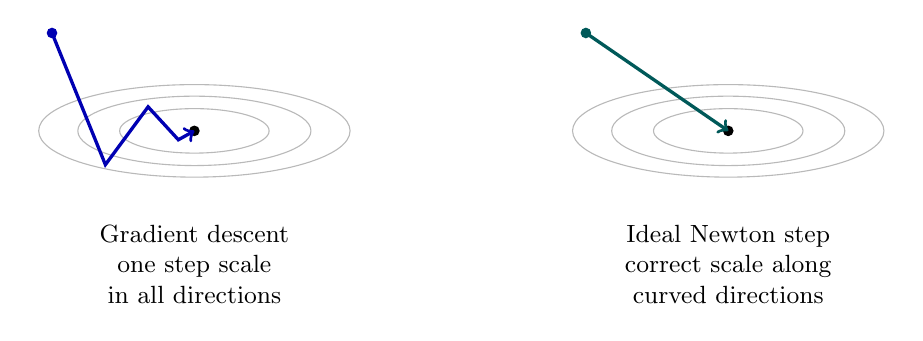
\begin{tikzpicture}[scale=1.13]
\begin{scope}[xshift=0cm]
\draw[gray!55] (0,0) ellipse (1.75 and .52);
\draw[gray!55] (0,0) ellipse (1.31 and .39);
\draw[gray!55] (0,0) ellipse (.84 and .25);
\fill (0,0) circle (1.7pt);
\draw[->,very thick,blue!70!black] (-1.6,1.1)--(-1.0,-.38)--(-.52,.27)--(-.18,-.10)--(0,0);
\fill[blue!70!black] (-1.6,1.1) circle (1.7pt);
\node[font=\small,align=center,text width=4.0cm] at (0,-1.5) {Gradient descent\\one step scale in all directions};
\end{scope}
\begin{scope}[xshift=6.0cm]
\draw[gray!55] (0,0) ellipse (1.75 and .52);
\draw[gray!55] (0,0) ellipse (1.31 and .39);
\draw[gray!55] (0,0) ellipse (.84 and .25);
\fill (0,0) circle (1.7pt);
\draw[->,very thick,teal!70!black] (-1.6,1.1)--(0,0);
\fill[teal!70!black] (-1.6,1.1) circle (1.7pt);
\node[font=\small,align=center,text width=4.0cm] at (0,-1.5) {Ideal Newton step\\correct scale along curved directions};
\end{scope}
\end{tikzpicture}
\caption{Illustrative paths on the same narrow quadratic valley. Newton uses cross-direction curvature to correct the step; stochastic, nonquadratic losses do not generally permit a single-step solution.}
\end{figure}

A dense Hessian has $N_{\text{parameters}}^2$ entries, so storing or factoring it is generally impractical for large neural networks.
Much of second-order optimisation research is therefore about \emph{which approximation is cheap enough to be useful}.

\paragraph{L-BFGS} avoids the full Hessian by keeping a short history of parameter changes and gradient changes, from which it builds an approximate inverse-curvature action.
It can be effective for smaller smooth problems with reliable objective evaluations; its gradient history is less reliable with very noisy mini-batches, and line searches may require extra forward/backward passes.

\paragraph{Gauss--Newton} is useful when the objective is built from residual errors.
For $\mathcal L(\theta)=\frac12\|r(\theta)\|^2$, it approximates the Hessian by
\[
\underbrace{\nabla_\theta^2\mathcal L(\theta)}_{\text{full Hessian}}
\quad\approx\quad
\underbrace{\left(\frac{\partial r}{\partial\theta}\right)^\top
\left(\frac{\partial r}{\partial\theta}\right)}_{\text{positive-semidefinite Gauss--Newton curvature}}.
\]
This drops second derivatives of the residuals and gives a positive-semidefinite curvature model, but the approximation may be poor far from a good fit.

\paragraph{Hessian-vector products} calculate $\nabla_\theta^2\mathcal L\,v$ without constructing the whole Hessian, allowing iterative linear solvers to approximate Newton-like directions.
The memory cost improves, but each iterative solve still requires additional differentiation work.

\paragraph{K-FAC} approximates layerwise curvature using Kronecker products of smaller matrices, giving an approximate natural-gradient direction based on Fisher information rather than the full Hessian.
\paragraph{Shampoo} uses matrix preconditioners along tensor dimensions so an update incorporates relationships within rows/columns or other tensor axes, rather than only elementwise scale.

\paragraph{Sophia} uses an inexpensive estimate of diagonal Hessian curvature and clips scaled coordinate updates.
It is more explicitly curvature-based than Adam, while deliberately giving up the cross-parameter information of a dense Newton step.

\begin{center}
\small
\begin{tabularx}{.97\linewidth}{@{}L{.19\linewidth}L{.27\linewidth}YY@{}}
\toprule
\textbf{Method} & \textbf{Geometry retained} & \textbf{Benefit} & \textbf{Cost / failure mode} \\
\midrule
Adam / RMSProp & Squared-gradient scale per coordinate & Cheap adaptive first-order updates & No cross-coordinate coupling \\
Newton / damped Newton & Full local Hessian & Corrects direction and scale for local curvature & Quadratic state; nonconvex curvature \\
L-BFGS & Recent changes in slope & No dense stored Hessian & Gradient noise / line-search overhead \\
Gauss--Newton & Jacobian-derived curvature & PSD approximation for residual objectives & Residual-model approximation \\
K-FAC / Shampoo & Structured layer/tensor preconditioner & Retains some coordinate interactions & Matrix state and operations \\
Sophia & Estimated diagonal Hessian & Curvature-adaptive scaling & No off-diagonal coupling; clipped steps \\
\bottomrule
\end{tabularx}
\end{center}


\section{Practical Points}

\subsection{Learning-Rate Schedules}
\label{sec:optimisation-learning-rate-schedules-and-warmup}
We can schedule Larning rate changes within a training run:
\begin{itemize}
    \item \textbf{Warmup} increases it gradually while gradient scales and optimiser state settle,
    \item \textbf{decay} reduces later changes,
    \item \textbf{cosine} decay changes it smoothly,
    \item \textbf{plateau} schedules react to a monitored metric
    \item \textbf{inverse-square-root}, 
\end{itemize}


\figpdf[.83\textwidth]{learning_rate_schedules}{Common relative learning-rate schedules: warmup, constant rate, cosine decay and a discrete step decay. The schedule is part of the optimiser, not a cosmetic setting.}



\subsection{Gradient Clipping}
A large gradient can cause instability in the loss function, and so we often clip off the tops of gradients to make sure they're always less than a threshold. 

\paragraph{Global-Norm } scales the entire gradient when its norm exceeds a threshold:
\[
    \underbrace{g_t^{\text{clipped}}}_{\text{gradient passed to optimiser}}
    =
    \underbrace{g_t}_{\text{computed gradient}}
    \min\!\left(1,\frac{\underbrace{c}_{\text{maximum norm}}}{\|g_t\|+\epsilon}\right).
\]
Unlike clipping each coordinate separately, global-norm clipping preserves the gradient's direction when it is clipped.

\begin{calloutpractical}
    For mixed-precision training, unscale gradients before clipping so the threshold applies to their real scale.
\end{calloutpractical}

\subsection{Gradient Accumulation}
\label{sec:optimisation-gradient-accumulation-and-mixed-precision}
Accelerator memory can limit the number of examples resident during one forward/backward pass.
\textbf{Gradient accumulation} runs several microbatches, adds or averages their gradients and updates parameters once:
\[
\underbrace{N_{\text{effective batch}}}_{\text{examples per update}}
=
\underbrace{N_{\text{microbatch}}}_{\text{resident examples}}
\times
\underbrace{N_{\text{accumulation steps}}}_{\text{passes per update}}
\times
\underbrace{N_{\text{data-parallel workers}}}_{\text{parallel workers}}.
\]
For a mean loss, each microbatch contribution must be weighted so the accumulated gradient represents the intended effective-batch average.
Accumulation reduces peak activation memory.

\begin{figure}[htbp]
\centering
\begin{tikzpicture}[node distance=8mm and 8mm]
\node[flow] (m1) {Microbatch 1\\forward + backward};
\node[flow,right=of m1] (m2) {Microbatch 2\\forward + backward};
\node[flow,right=of m2] (mk) {$\cdots$\\accumulate};
\node[yesbox,right=of mk] (step) {One optimiser\\step};
\draw[arr] (m1)--(m2);
\draw[arr] (m2)--(mk);
\draw[arr] (mk)--(step);
\end{tikzpicture}
\caption{Original accumulation data flow: several smaller backward passes contribute to one effective-batch gradient and one parameter update.}
\end{figure}
\begin{calloutmemoryhook}
Accumulation reduces each batches memory.
\end{calloutmemoryhook}

\subsection{Mixed precision} performs suitable computation and storage in lower precision while keeping numerically sensitive quantities, often optimiser state, at higher precision.
FP16 offers more precision than BF16 but a much narrower exponent range.
BF16 tolerates a larger dynamic range, often avoiding the need for FP16-style loss scaling.
FP16 loss scaling temporarily multiplies the loss to keep small gradients representable, then unscales gradients before clipping and updating.
Lower precision usually reduces activation memory and bandwidth, but it does not guarantee a proportional speed-up if the workload is limited by launches, communication or unsupported operations (see the hardware chapter).

\begin{calloutmemoryhook}
    Mixed precision reduces bytes per tensor value.
\end{calloutmemoryhook}

\subsection{Diagnosing Problems}

\begin{center}
    \small
    \begin{tabularx}{.96\linewidth}{@{}L{.29\linewidth}YY@{}}
    \toprule
    \textbf{Observed behaviour} & \textbf{Likely variable to test} & \textbf{Interpretation / measurement} \\
    \midrule
    Loss diverges or oscillates & Learning rate, warmup, clipping & Inspect gradient/update norms and non-finite values \\
    Loss falls slowly in a narrow valley & Momentum or curvature scaling & Compare validation loss per unit compute \\
    Early progress, then stalls & Schedule; AdaGrad state; batch size & Compare effective learning rates and noise \\
    GPU memory exhausted & Microbatch, accumulation, precision, optimiser state & Separate activation, parameter and optimiser-state memory \\
    Training improves, validation degrades & Decay, data, regularisation, early stopping & Generalisation problem, not necessarily optimiser failure \\
    \bottomrule
    \end{tabularx}
\end{center}

\begin{calloutdegreeofexperiment}
Vary optimiser, learning-rate schedule, batch size, momentum/scale decay, gradient clipping, numerical precision, accumulation, weight decay and which parameter groups use each update rule.
\end{calloutdegreeofexperiment}

\section{Full Training Loop}
\label{sec:optimisation-the-full-training-loop}
The mathematical and systems choices above decompose to:
\begin{lstlisting}
optimizer.zero_grad()           # clear previous gradients
for inputs, targets in train_loader:
    predictions = model(inputs) # forward pass (optionally BF16/FP16)
    loss = loss_fn(predictions, targets) / accumulation_steps
    loss.backward()              # accumulate gradients

    if accumulation_boundary or final_batch:
        if FP16 loss scaling:
            unscale_gradients()
        clip_grad_norm_(model.parameters(), max_norm)
        optimizer.step()        # update parameters (AdamW decay here)
        optimizer.zero_grad()   # reset accumulated gradients
        scheduler.step()        # if scheduled per update
\end{lstlisting}
\textbf{Accumulation} delays the optimiser step until several backward passes have contributed gradients.
\textbf{Clipping} acts on the accumulated, unscaled gradients immediately before the optimiser step.
\textbf{Mixed precision} changes the forward/backward numerical representation.
FP16 may require loss scaling, while BF16 generally does not.
A scheduler is advanced after successful updates, per epoch or per validation metric according to its definition.